\documentclass[12pt, twoside]{article}
\usepackage[letterpaper, margin=1in, headsep=0.5in]{geometry}
\usepackage[english]{babel}
\usepackage[utf8]{inputenc}
\usepackage{amsmath}
\usepackage{amsfonts}
\usepackage{amssymb}
\usepackage{tikz}
%\usetikzlibrary{quotes, angles}

\usepackage{graphicx}
\usepackage{enumitem}
\usepackage{multicol}

\usepackage{fancyhdr}
\pagestyle{fancy}
\fancyhf{}
\renewcommand{\headrulewidth}{0pt} % disable the underline of the header

\fancyhead[RE]{\thepage \\ Name: \hspace{3cm}}
\fancyhead[RO]{\thepage \\ Name: \hspace{3cm}}
\fancyhead[L]{BECA / Dr. Huson / 10th Grade Geometry\\* 17 January 2019}

\begin{document}
\subsubsection*{Homework: Regents Pre-test} %Version 1

Use the last four digits of your student number as your Gradecam ID. Write the number and bubble in your ID (1 point).\\[0.5cm]


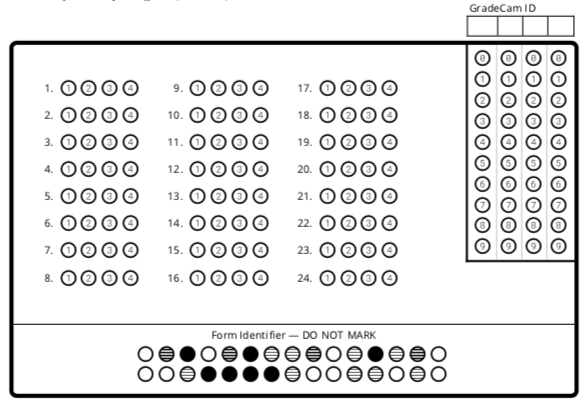
\includegraphics[width=1.0\textwidth]{6-10HW_gradecam24-v1.png} \\ \vspace{0.5cm}

\newpage
\subsubsection*{Homework: Regents Pre-test} %Version 2

Use the last four digits of your student number as your Gradecam ID. Write the number and bubble in your ID (1 point).\\[0.5cm]


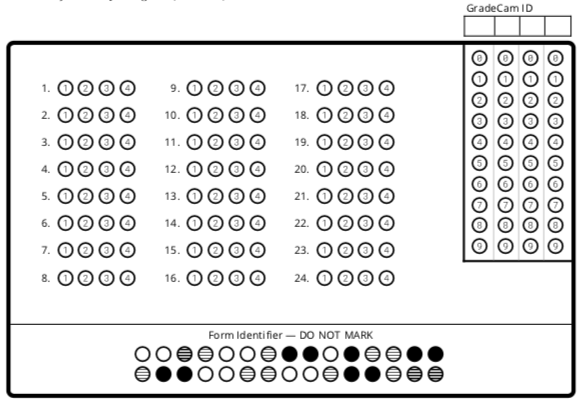
\includegraphics[width=1.0\textwidth]{6-10HW_gradecam24-v2.png} \\ \vspace{0.5cm}


\end{document}
